There are multiple ways to approach discretizing the ellipse, the most apparent of which being
\begin{equation}\label{eq:parametric_ellipse}
  \xtt = a\cos{t} + ib\sin{t}, \qquad t \in [0, 2\pi),
\end{equation}
where the parameter $t$ is the very same as $\eta$, called the \emph{eccentric} variable.
It is indeed related, as is clear upon considering $\tan{t}$.
This value is equal to $\sfrac{az}{bx}$, by the geometric interpretation of the tangent, where $\xtt = x + iz$.
For a polar representation
\begin{equation}\label{eq:polar_ellipse}
\xtt = r\cos{\theta} + ir\sin{\theta}, \qquad \theta \in [0, 2\pi),
\end{equation}
we find that
\[
\tan{t} = \sfrac{a}{b} \tan{\theta}, \quad r(\theta) = \frac{ab}{\sqrt{b^2 \cos^2{\theta} + a^2 \sin^2{\theta}}}.
\]
We may discretize $\theta$ into a \texttt{linspace}, an array of equally spaced points of the interval $[0, 2\pi)$, and plot the coordinates of the ellipse according to equation \eqref{eq:polar_ellipse}, as is done in figure \ref{fig:polar_ellipse} below.
\begin{Figure}
  \centering
  \scalebox{1}{%
    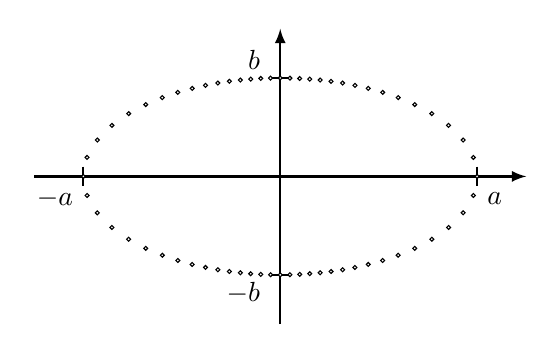
\begin{tikzpicture}
  \begin{scope}[scale = 2.5]
    \def\majradius{1}
    \def\minradius{0.5}
    \def\slingringsmonn{.25}
    \draw[-latex, thick] ({-\majradius - \slingringsmonn}, 0)--({\majradius + \slingringsmonn}, 0);
    \draw[-latex, thick] (0, {-\minradius - \slingringsmonn})--(0, {\minradius + \slingringsmonn});
    \draw[thick] ({-\majradius}, .05)--({-\majradius}, -.05) node[below = 1ex, left]{$-a$};
    \draw[thick] ({\majradius}, .05)--({\majradius}, -.05) node[below = 1ex, right]{$a$};
    \draw[thick] (.05, {\minradius})--(-.05, {\minradius}) node[above = 1.5ex, left]{$b$};
    \draw[thick] (.05, {-\minradius})--(-.05, {-\minradius}) node[below = 1.5ex, left]{$-b$};
    \def\numbernodes{64}
    \foreach \i in {0, ..., \numbernodes}
      \pgfmathsetmacro\teta{2 *\i * pi / \numbernodes}
      \def\radius{(\majradius*\minradius)/sqrt(\minradius^2 * (cos(\teta r))^2 + \majradius^2 * (sin(\teta r))^2)}
      \draw[fill = white] ({\radius*cos(\teta r)}, {\radius*sin(\teta r)}) circle (.01);
  \end{scope}
\end{tikzpicture}

  }
  \captionsetup{type = figure}
  \caption{Ellipse parametrized with the polar variable $\theta$, according to equation \eqref{eq:polar_ellipse}.}
  \label{fig:polar_ellipse}
\end{Figure}
We see that the points tend to accumulate at the top of the ellipse, which indeed makes sense.
As we change the polar angle by an equal amount counter-clockwise, the arc length drawn out between points will diminish towards $\sfrac{\pi}{2}$.
This is illustrated in figure \ref{fig:polar_arc_length_ellipse} below, where points on the ellipse for integer multiples of $\sfrac{\pi}{8}$ are plotted in the first quadrant.
\begin{Figure}
  \centering
  \scalebox{1}{%
    \begin{tikzpicture}
  \begin{scope}[scale = 5]
    \def\slingringsmonn{.2}
    \def\majorradius{1}
    \def\minorradius{.5}
    \draw[thick, -latex] ({-\slingringsmonn}, 0)--({\majorradius + \slingringsmonn}, 0);
    \draw[thick, -latex] (0, {-\slingringsmonn})--(0, {\minorradius + \slingringsmonn});
    \draw[thick] (\majorradius, .05)--(\majorradius, -.05) node[below]{$a$};
    \draw[thick] (.05, \minorradius)--(-.05, \minorradius) node[left]{$b$};
    \foreach \i in {0, ..., 4}
      \pgfmathsetmacro\teta{\i * pi / 8}
      \def\radius{(\majorradius*\minorradius)/sqrt(\minorradius^2 * (cos(\teta r))^2 + \majorradius^2 * (sin(\teta r))^2)}
      \draw[fill = white] ({\radius*cos(\teta r)}, {\radius*sin(\teta r)}) circle (.01);
  \end{scope}
\end{tikzpicture}

  }
  \captionsetup{type = figure}
  \caption{Demonstration that the arc length between points decreases clockwise in the first quadrant as the polar angle $\theta$ approaches $\sfrac{\pi}{2}$.}
  \label{fig:polar_arc_length_ellipse}
\end{Figure}
This is not the case for the ellipse discretized according to equation \eqref{eq:parametric_ellipse}, using the eccentric variable $t$, as is seen in figure \ref{fig:eccentric_ellipse} below.
\begin{Figure}
  \centering
  \scalebox{1}{%
    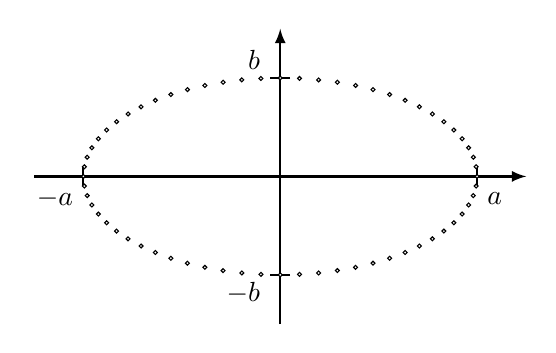
\begin{tikzpicture}
  \begin{scope}[scale = 2.5]
    \def\majradius{1}
    \def\minradius{.5}
    \def\slingringsmonn{.25}
    \draw[-latex, thick] ({-\majradius - \slingringsmonn}, 0)--({\majradius + \slingringsmonn}, 0);
    \draw[-latex, thick] (0, {-\minradius - \slingringsmonn})--(0, {\minradius + \slingringsmonn});
    \draw[thick] ({-\majradius}, .05)--({-\majradius}, -.05) node[below = 1ex, left]{$-a$};
    \draw[thick] ({\majradius}, .05)--({\majradius}, -.05) node[below = 1ex, right]{$a$};
    \draw[thick] (.05, {\minradius})--(-.05, {\minradius}) node[above = 1.5ex, left]{$b$};
    \draw[thick] (.05, {-\minradius})--(-.05, {-\minradius}) node[below = 1.5ex, left]{$-b$};
    \def\numbernodes{64}
    \foreach \i in {1, ..., \numbernodes}
      \draw[fill = white] ({\majradius*cos(2*\i*pi/\numbernodes r)}, {\minradius*sin(2*\i*pi/\numbernodes r)}) circle (.01);
  \end{scope}
\end{tikzpicture}

  }
  \captionsetup{type = figure}
  \caption{Ellipse parametrized with the eccentric variable $t$, according to equation \eqref{eq:parametric_ellipse}.}
  \label{fig:eccentric_ellipse}
\end{Figure}
